%!TEX root = paper.tex
%%%%%%%%%%%%%%%%%%%%%%%%%%%%%%%%%%%%%%%%%%%%%%%%%%%%%%%%%%%%%%%%%%%%%%%%%%%%%%%



\section{Fragestellungen}

\begin{itemize}
	\item Kostenmodell für Cloud Gaming Provider?
	\item Attraktivität für “Core Gamer”?
	\item Wieviel ist eine NutzerIn bereit für einen Streaming Service mit einem bestimmten Spieleangebot und einer bestimmten Streaming- Qualität (Video-Qualität, Latenz, Grafikeinstellungen des Spiels) zu zahlen?
\end{itemize}

Netflix-Analogie? 


\section{Kostenfaktoren}

\subsection{Cloud Gaming Provider}

\subsubsection{CAPEX}

\begin{itemize}
	\item Regionale Data Center
	\item Gaming Server (GPU-Enabled)
	\item Entwicklungskosten für Software-Plattform(?)
\end{itemize}

\subsubsection{OPEX}

\paragraph{Verkehrsvolumen}

\begin{itemize}
	\item Internetanbindung?
	\item Caching of basic resources is probably not applicable?
\end{itemize}

\paragraph{Serverlaufzeiten}

\begin{itemize}
	\item Energie
	\item Verschleiß
	\item Wartungs- und Betriebspersonal oder Anmietung
	\item Frage: Rechnet sich Anmietung von Ressourcen bei großen generischen Rechenzentren? Annahme nein, da man selbst ein großer Anbieter wäre u. die Margin wegfallen. Auf der anderen Seite gibt es Hardware die für Games im Serverbereich besser skalieren? Wenn ja, kann umso mehr kein generischer Anbieter die Lösung sein
\end{itemize}

\paragraph{Spiele-Lizenzen und -Adaptionskosten (?)}
Modelannahme: Kosten pro Nutzung (realistisch eher in Blöcken verrechnet)




\section{Data}

Bereits Gesammelte Daten

\subsection{Steam API + SteamSpy Datensätze+Graphen}
\url{https://github.com/mas-ude/steam-data-stats} Steam + SteamSpy REST API Datensammler + ein paar Graphplotter (und eher ergebnislose Clustering-Versuche); für sinnvolle Analsyen müsste man dazu aber viel häufiger Datensätze generieren. Beispielausgaben:

CDF der Preise auf Steam (Juli ‘15) \ref{fig:steam-prices}

\begin{figure}[!t]
	\centering
	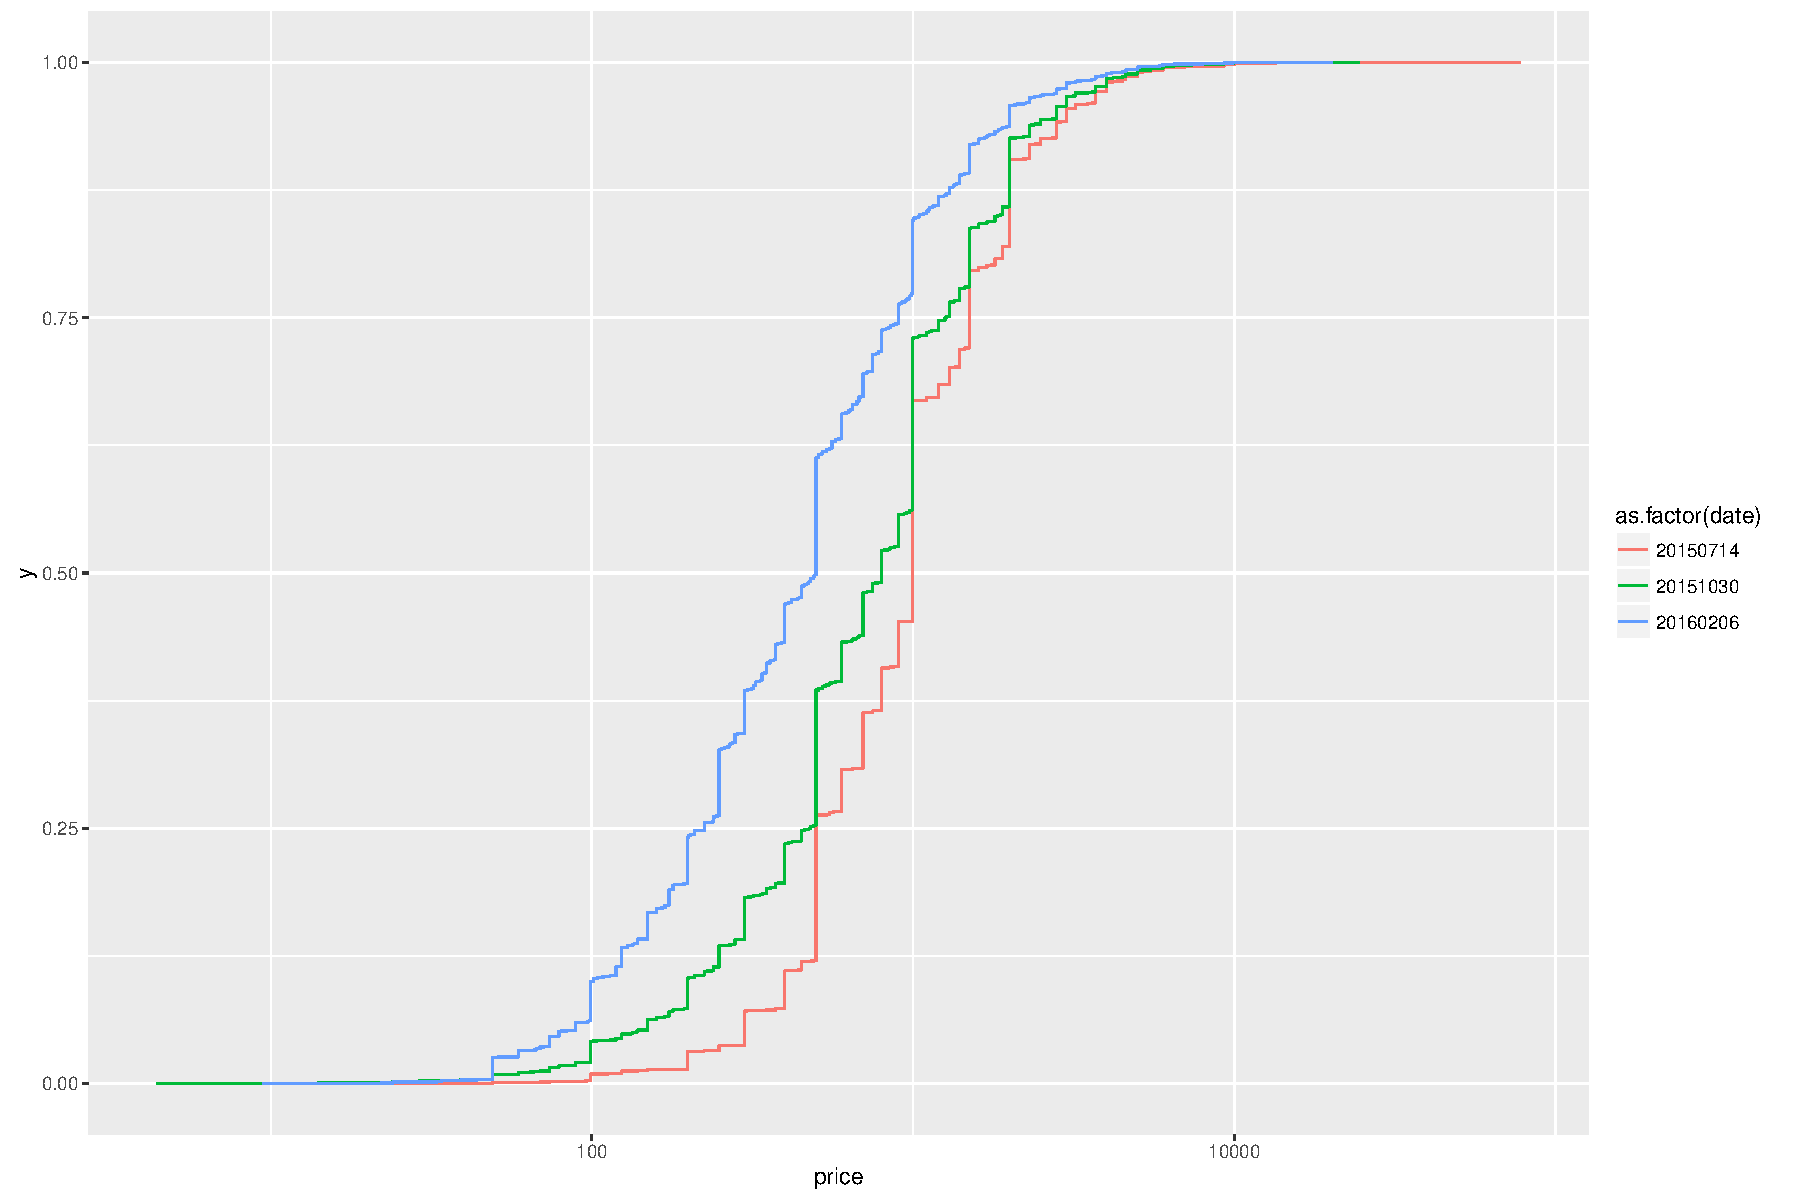
\includegraphics[width=1.0\columnwidth]{images/steam-prices.pdf}
	\caption{CDF of games on the steam platform at two distinct dates.}
\label{fig:steam-prices}
\end{figure}

Violinenplot der durchschnittlichen Spielzeit aufgeteilt auf unterschiedliche Preiskategorien. \ref{fig:steam-cost-vs-playtime-violin}

\begin{figure}[!t]
	\centering
	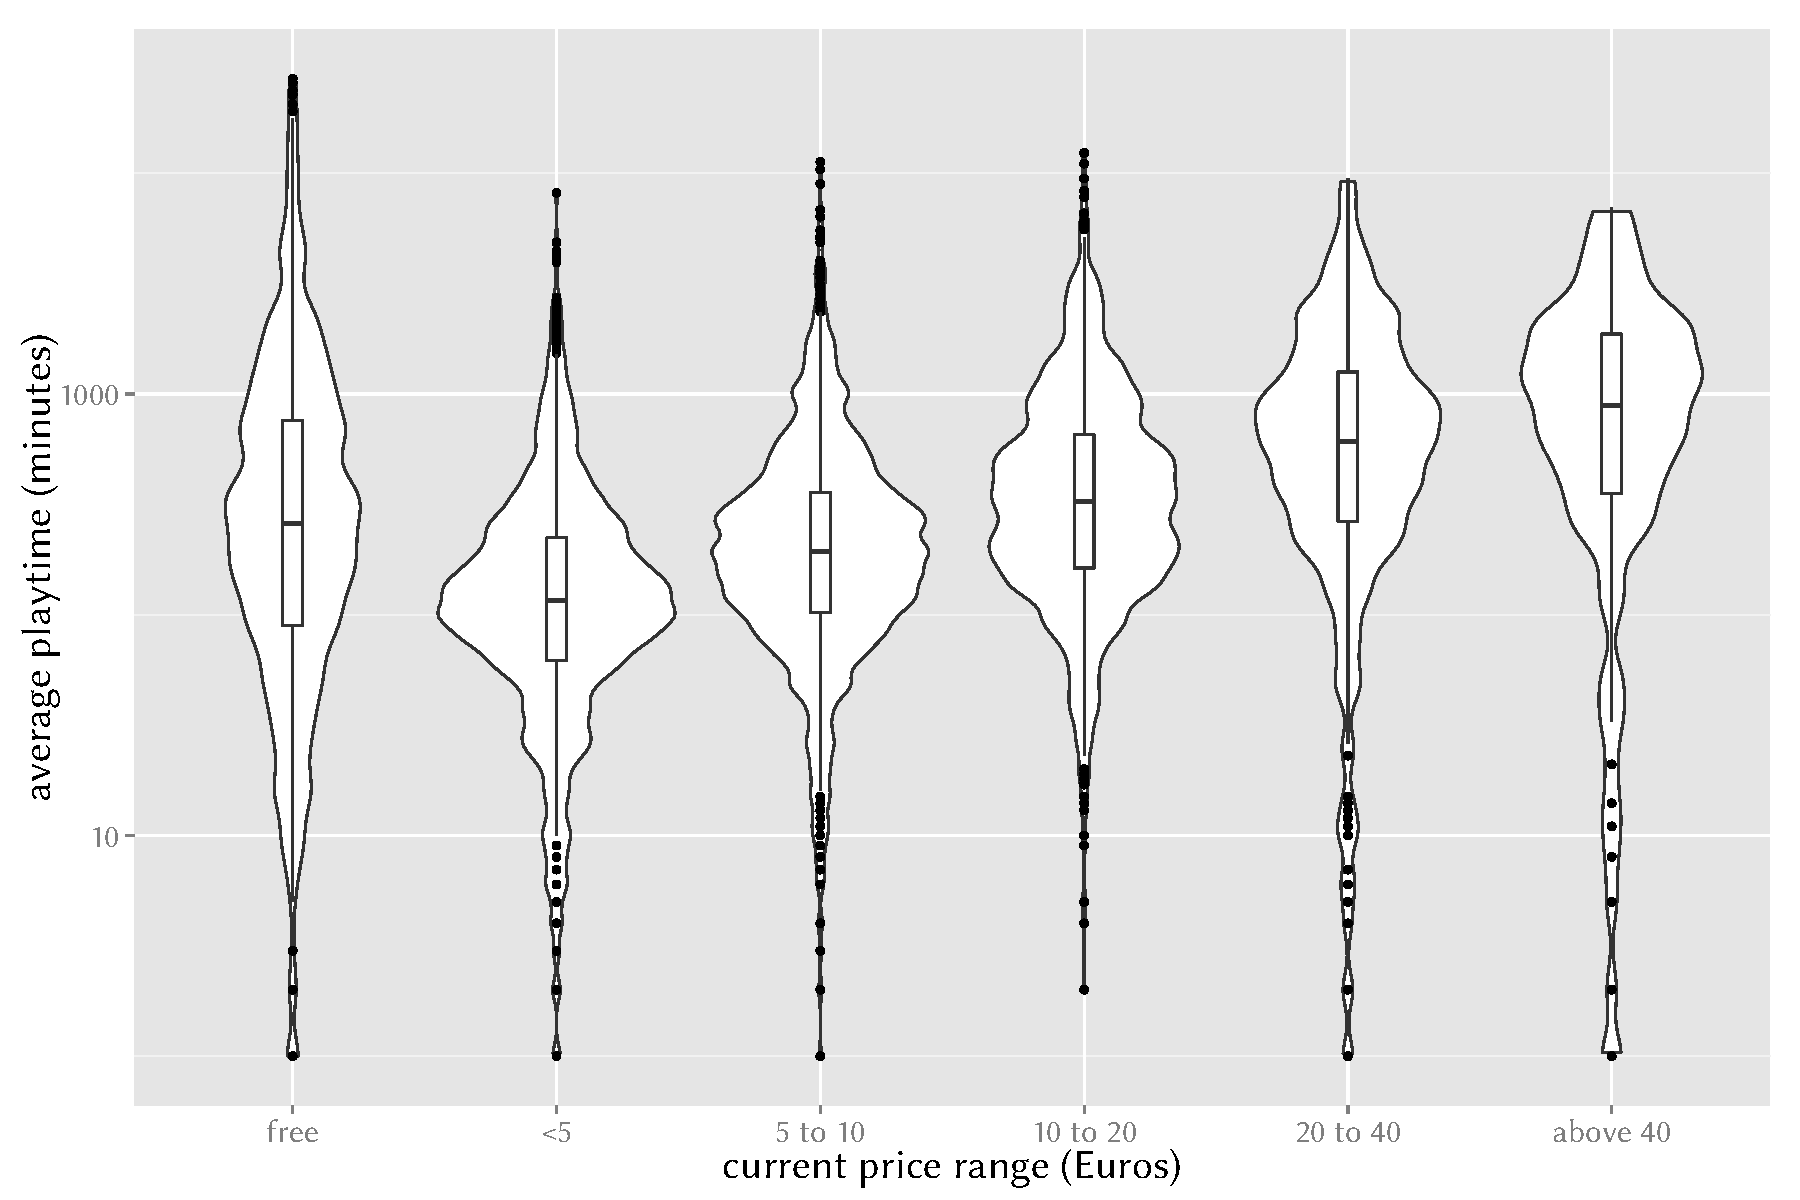
\includegraphics[width=1.0\columnwidth]{images/steam-cost-vs-playtime.pdf}
	\caption{Violin plot of the average playtime (as recorded by SteamSpy) of games categorized by their prices.}
\label{fig:steam-cost-vs-playtime-violin}
\end{figure}



\subsection{platform-market-comparison/games-per-year.R}

 hat den ersten Versuch einer Nutzenrechnung für Spieler auf verschiedenen Plattformen. Script könnte leicht angepasst und erweitert werden. Beispielausgabe \ref{fig:gamesperyear-over-budget}, \ref{fig:steam-prices}

\begin{figure}[!t]
	\centering
	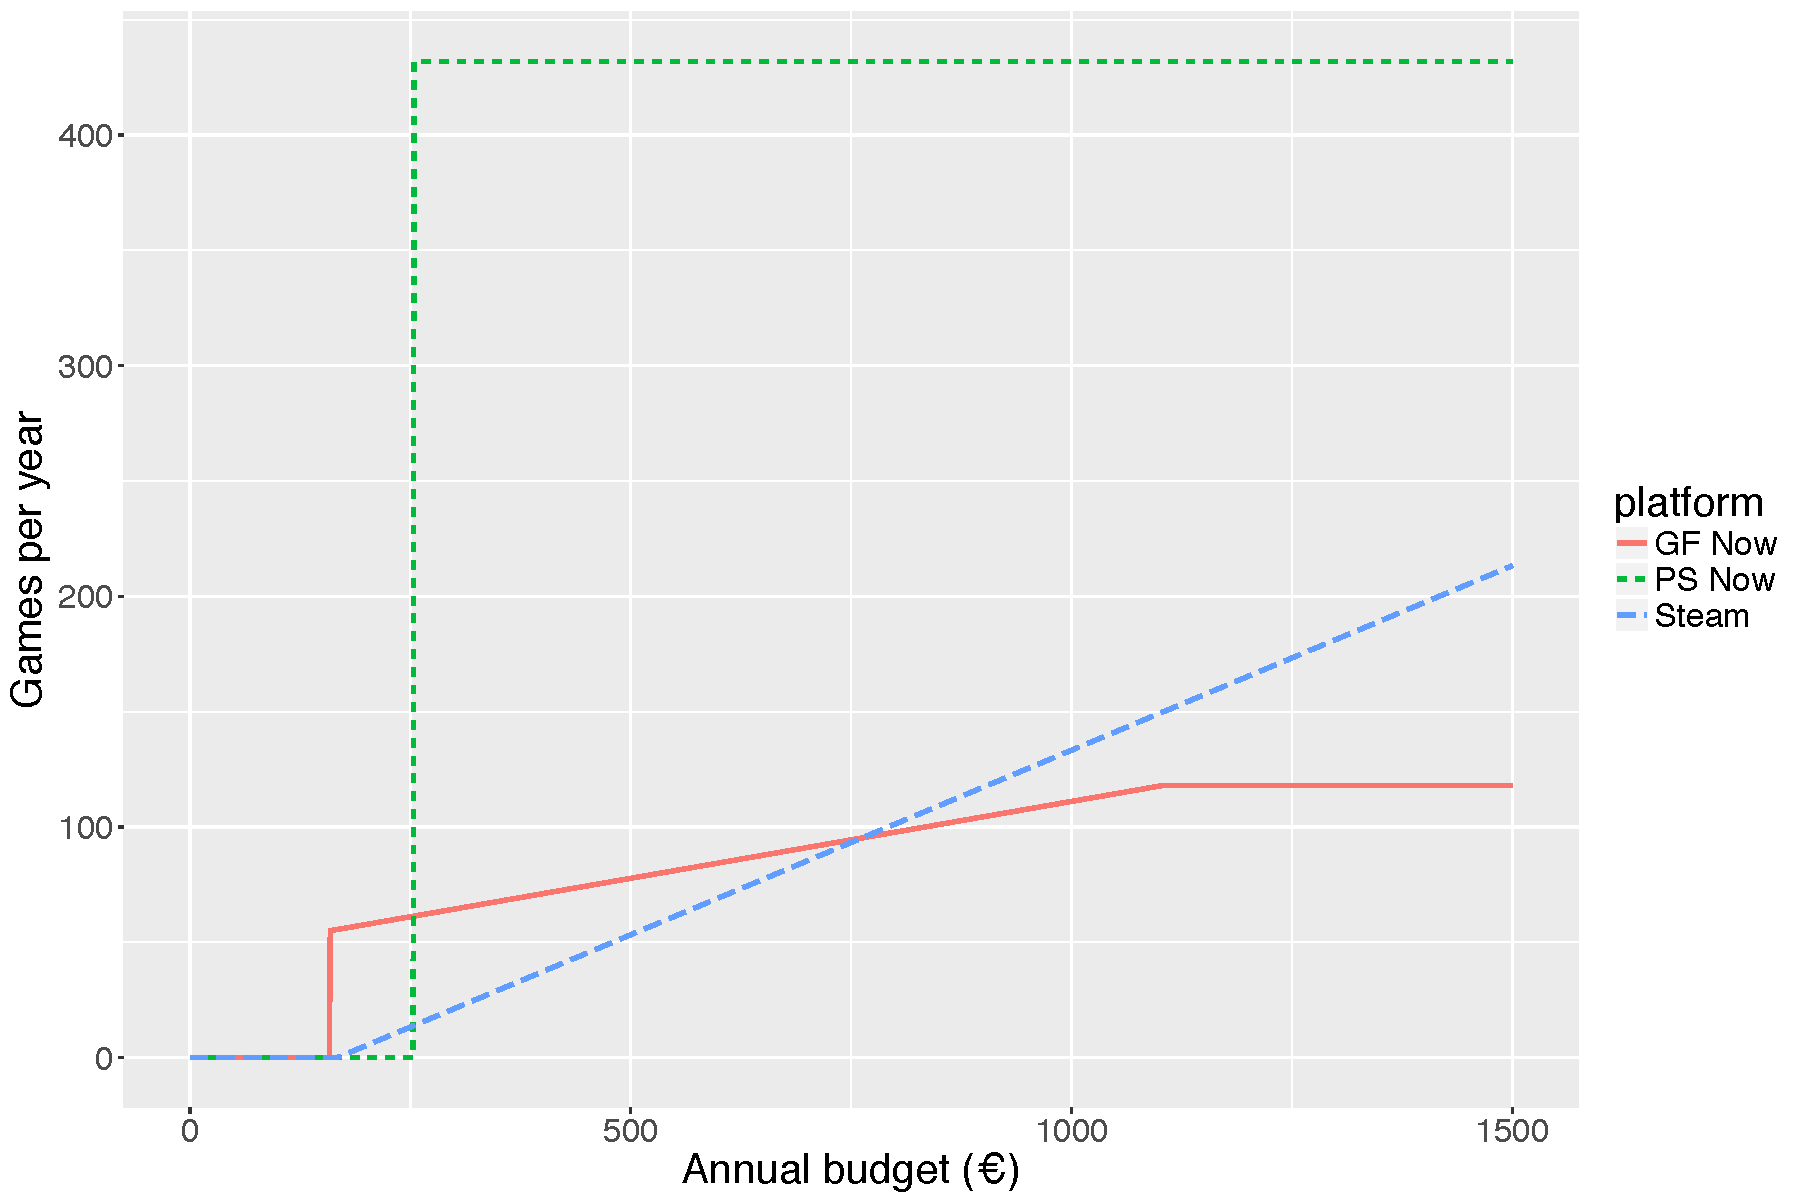
\includegraphics[width=1.0\columnwidth]{images/gamesperyear-over-budget.pdf}
	\caption{Models for several platforms showing the number of games per year that can be bought with a specific \$ budget.}
\label{fig:gamesperyear-over-budget}
\end{figure}

\begin{figure}[!t]
	\centering
	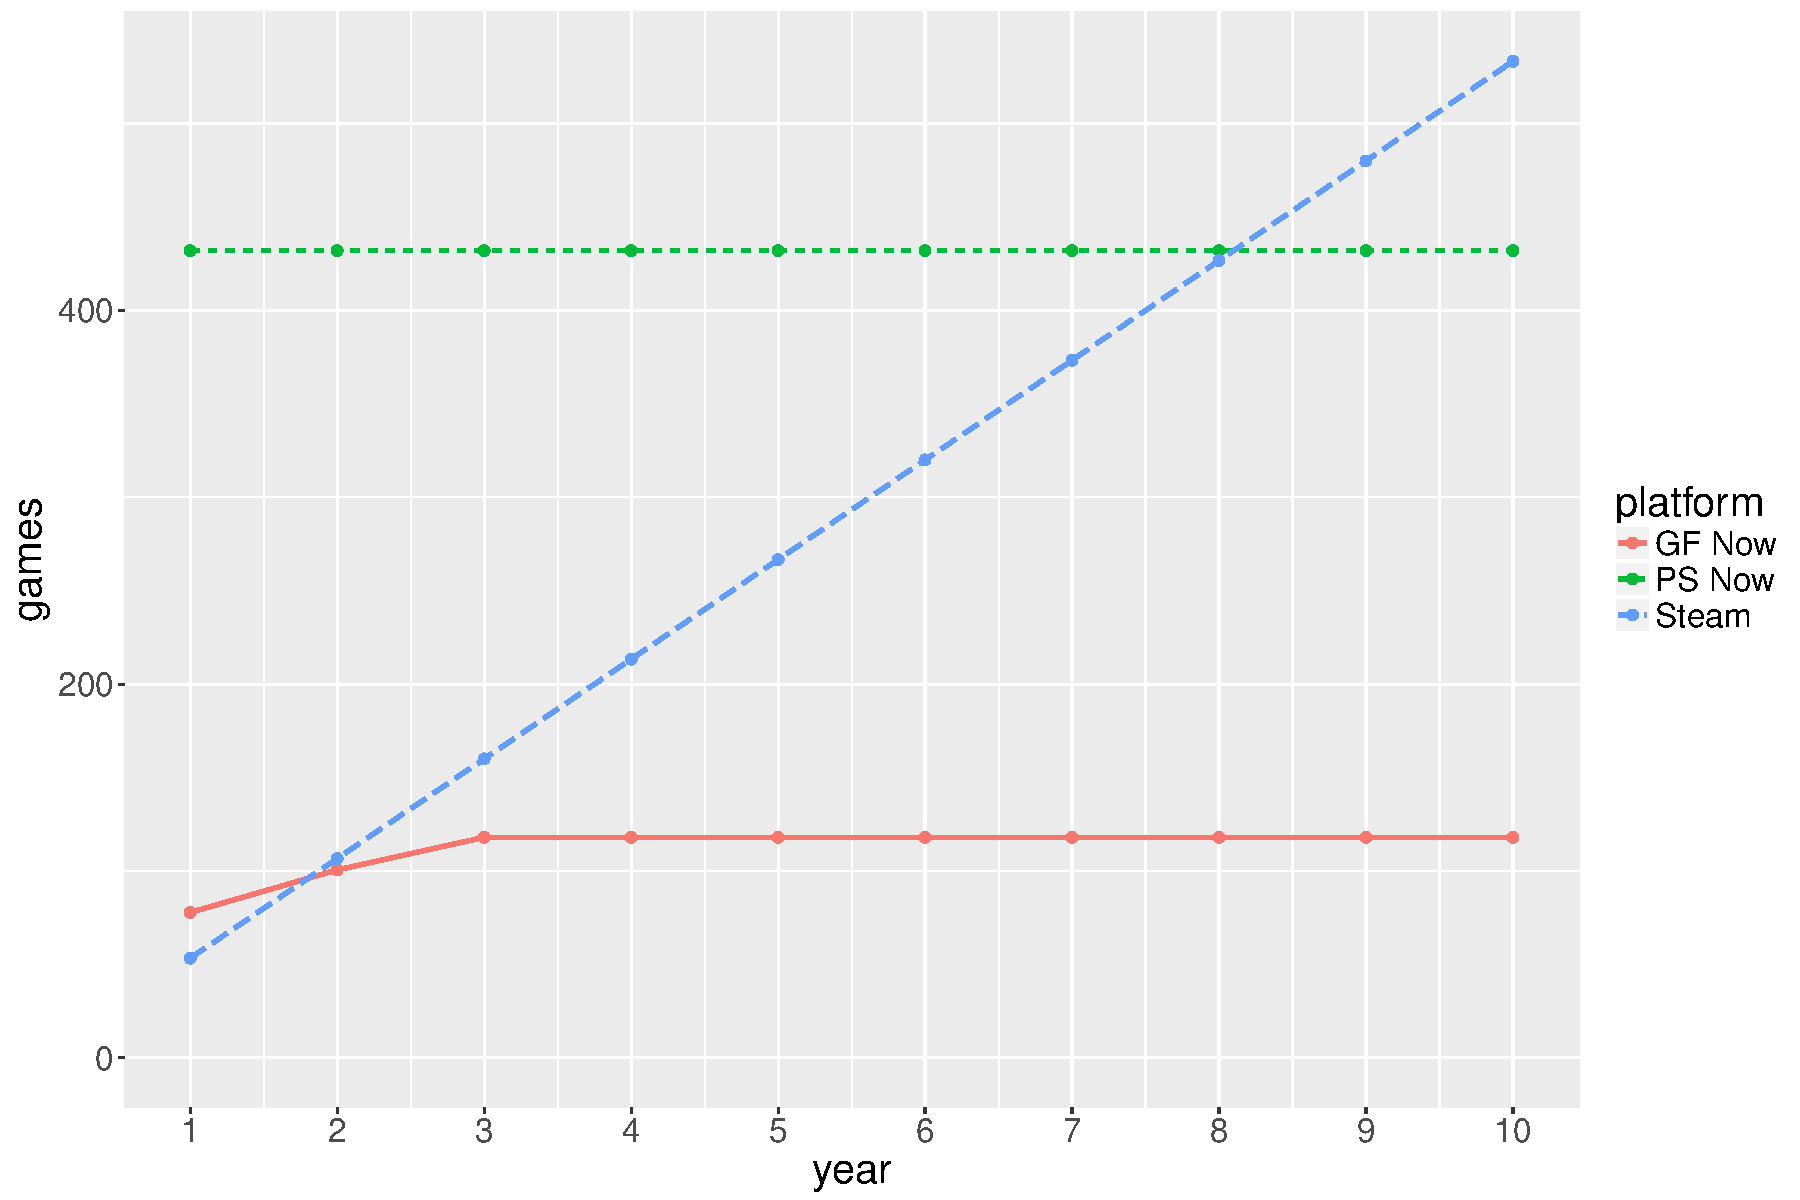
\includegraphics[width=1.0\columnwidth]{images/games-over-year.pdf}
	\caption{Models for several platforms showing the number of games that can be bought over the years subscribed to / using this service.}
\label{fig:games-over-years}
\end{figure}


\subsection{E2E Lag}
End-to-End Lag Model and Simulation in R. Now a standalone (submitted) paper at \url{https://github.com/mas-ude/onlinegame-lag-sim}. Can be referenced to argue the need for low E2E lag (meaning low network delay, but also the need for high fps).



\subsection{Other Useful Data for Model Creation}

\begin{itemize}
	\item Game costs (current cost possible via Steam dataset; historic price data more difficult)
	\item Length of games (either via howlongtobeat dataset (via \url{https://github.com/mas-ude/gamelengths-scraper}), SteamSpy data, or could also additionally manually parse more Steam data)
	\item Gaming score/ratings/rankings (via Metacritic dataset (via \url{https://github.com/mas-ude/metacritic_scraper}), or might want to additionally scrape steam user review scores)
	\item Other popularity measures? (e.g. steamspy owner data?)
	\item Influence of E2E lag on games? (could be theorized indirectly through e2e lag sim + categorization attempts)
	\item Hardware requirements of games?
\end{itemize}


\section{Cloud Gaming Services}

\subsection{Individual Services and Their Price Models}
TODO: update and correct the information


\paragraph{NVIDIA Now}
\url{http://shield.nvidia.com/game-streaming-with-geforce-now}
Kosten

\$7.99/mo + 200\$/€++ Hardware

Started in parts of Europe in Q4/2015

Spieleangebot

\$x Spiele im Paket

 + weitere/neuere zusätzlich mit Einmalbetrag

Leistung
Bandbreite? 

\paragraph{Playstation Now}
Streaming von PS3 Spielen auf PS4 und andere Sony-Geräte (als Rückwärtskompatibiliätslösung)
Kosten

(US/UK only?) Deuschlandbeta seit ~Q4/2015

\$ /mo + 330\$/€ (PS4) oder Sony TV + Controller
Extrakosten/Tagesleihgebühren für bestimmte ``bessere'' Spiele


\subsection{Backend/Service Requirements and Demands}

\subsubsection{Hardware}

\url{https://www.nvidia.com/object/cloud-gaming-gpu-boards.html}
\url{https://www.nvidia.com/object/grid-technology.html}


\subsection{Models}

\subsubsection{Cost Model}

\paragraph{CAPEX}

Regionale Data Center => SERVER HARDWARE? (siehe unterhalb?)

Gaming Server (GPU-Enabled) => vermutlich ebenso aggregiert enthalten unten?

Entwicklungskosten für Software-Plattform(?) => noch nicht enthalten? Wie hoch sind die Anpassungskosten?

CAPEX in our case is a dimensioning problem.

CAPEX are typically used in the sense of depreciation costs. We have to define the runtime of hardware and calculate the cost per user and year to understand whether it is profitable on a per contract basis later on.

Probably we have to fill this model on a per regional data center perspective??

peak\_use = Users * peak\_load\_factor

peak\_resource\_demand = peak\_use * average\_resource\_demand

peak\_quality\_demand = peak\_use * overprovisioning

infrastructure\_cost = peak\_quality\_demand * investement\_per\_per\_resource\_unit

game\_adaptation\_costs = XXXXX => meine Vermutung: Integration über Prozentsatz am Licensing in OPEX leichter, da schätzbar?

Depreciation times in Germany for mainframes: 7 years [Quelle noch ausstaendig.. Gesetz?]
fm: I would argue that gaming servers lose their value much more quickly than regular servers: you won’t be able to run a current game on a 7-year old machine in a reasonable quality. At least the number of games will be very limited, reducing their value. 
You would probably need to mix in new hardware every 2-3 years.

Ok, but what’s the full cycle to completely swap the hardware or double it up? If it is 5-6 years, then the depreciation time is 5-6 years. If it is lower than that, we go lower etc. etc. It is fair to argue 7 years is too much, but the server might have a 7-year value if it is generic hardware that is just used for games. Otherwise the value has decreased to 0 in the 5-6 years range. I need to do some research here … :D

CAPEX\_per\_year = infrastructure\_cost / 7

CAPEX\_per\_contract = CAPEX\_per\_year / users 

Note: Users are kept static for the one-shot analysis. 


\paragraph{OPEX}

OPEX consists of several components: Network traffic generates costs (interconnection fees and/or wholesale Internet access fees); energy; maintenance (replacement units and cost to replace and monitor things); licensing (probably it’s a per year fee rather than a “purchase” => shift to CAPEX otherwise)

use\_time = users * avg\_time\_per\_year

energy\_cost = use\_time * avg\_energy\_demand * energy\_unit\_price

network\_cost = use\_time * avg\_network\_res\_demand * network\_unit\_price

maintenance\_cost = use\_time * feailure\_propability * failure\_cost (personnel; replacement\_units; etc.)

licensing = use\_time * license\_per\_use\_time

OPEX\_per\_year = energy\_cost + network\_cost + maintenance\_cost + licensing

OPEX\_per\_contract = OPEX\_per\_year / users


\paragraph{CUSTOMER COSTS / CONSUMER RATIONALE}

The customer pays the revenue (see below) + hardware costs. Substitutes (like Steam or classical console games) can be compared on this basis or on the revenue side to understand how much one can price for it.

200(++) for hardware but probably we can use the depreciation time of 4 years here. 
=> Hardware costs: 200 Euros / 5 = 40 Euros


End\_customer\_cost\_per\_year = R/users + 40

Now compare to alternatives. An alternative i is dominated by j if End\_customer\_cost\_per\_year ** i > End\_customer\_cost\_per\_year ** j

Alternative products are: Console games, PC games, steam, etc.

If no feasible revenue model can be found to both generate profit and to satisfy the customer rationale, the model is unsuccessful and does not stand the competition with substitutes.


\subsubsection{Revenue Model}

p\_year = p\_month * 12

p = p\_year / avg\_time\_per\_year

R = p  * use\_time OR p\_year * users


\subsubsection{Profit Model}

M(P=R-C)E

C = CAPEX\_per\_contract + OPEX\_per\_contract

R = see above...

M / E are external factors, which are probably not supported by equations. Let’s see later.


\section{Related Work}

TODO: Kategorisierung
TODO: Mehr Paper mit Fokus Cloud Gaming

``Gaming in the clouds: QoE and the users’ perspective'' (Michael Jarschel, Daniel Schlosser , Sven Scheuring , Tobias Hoßfeld): http://www.sciencedirect.com/science/article/pii/S0895717711007771 


``Modeling and Characterizing User Experience in a Cloud Server Based Mobile Gaming Approach'' (Shaoxuan Wang, Sujit Dey): http://esdat.ucsd.edu/projects/gaming/papers/globecom09.pdf


``A Comprehensive End-to-End Lag Model for Online and Cloud Video Gaming'' Metzger, Rafetseder, Schwartz, Hoßfeld, Networking 2016 (Submitted)

``On the Impact of Delay on Real-time Multiplayer Games'' \cite{Pantel:2002:IDR:507670.507674}

``The Effects of Loss and Latency on User Performance in Unreal Tournament 2003'' \cite{Beigbeder:2004:ELL:1016540.1016556}

``An experimental estimation of latency sensitivity in multiplayer Quake 3'' \cite{1266180}

``How Do New Visual Immersive Systems Influence Gaming QoE?'' \cite{7148110}

``The Impact of Video Encoding Parameters and Game Type on QoE for Cloud Gaming: a Case Study using the Steam Platform'' \cite{slivarimpact}

``QoE Assessment of Interactivity and Fairness in First Person Shooting with Group Synchronization Control'' \cite{Ida:2010:QAI:1944796.1944806}

``A Method For Feedback Delay Measurement Using a Low-cost Arduino Microcontroller'' \cite{beyermethod}

``Assessing the Impact of Game Type, Display Size and Network Delay on Mobile Gaming QoE'' \cite{beyer2014typedisplaydelayimpact}

``Using Electroencephalography and Subjective Self-Assessment to Measure the Influence of Quality Variations in Cloud Gaming'' \cite{beyerusing}

``Towards a New {ITU-T} Recommendation for Subjective Methods Evaluating Gaming {QoE}'' \cite{mollertowards}

``Kahawai: High-Quality Mobile Gaming Using GPU Offload'' \cite{Cuervo:2015:KHM:2742647.2742657}

``Outatime: Using Speculation to Enable Low-Latency Continuous Interaction for Mobile Cloud Gaming'' \cite{Lee:2015:OUS:2742647.2742656}

``Addressing Response Time and Video Quality in Remote Server Based Internet Mobile Gaming'' \cite{5506572}

``Are all games equally cloud-gaming-friendly? An electromyographic approach'' \cite{6404025}

``Subjective Evaluation of Latency and Packet Loss in a Cloud-Based Game'' \cite{6614351}

``Adaptive Mobile Cloud Computing to Enable Rich Mobile Multimedia Applications'' \cite{6413270}

``Placing Virtual Machines to Optimize Cloud Gaming Experience'' \cite{6853364}

``On frame rate and player performance in first person shooter games'' \cite{claypool2007}

``Cloud gaming: architecture and performance'' \cite{6574660}

``Latency and Player Actions in Online Games'' \cite{Claypool:2006:LPA:1167838.1167860}

``How Sensitive Are Online Gamers to Network Quality?'' \cite{Chen:2006:SOG:1167838.1167859}

``Security issues in online games'' \cite{doi:10.1108/02640470210424455}

``A Measurement Study Regarding Quality of Service and Its Impact on Multiplayer Online Games'' \cite{Bredel:2010:MSR:1944796.1944797}

``Empirical study of subjective quality for Massive Multiplayer Games'' \cite{4604397}

``Effect of Network Quality on Player Departure Behavior in Online Games'' \cite{4591393}

``On the Quality of Service of Cloud Gaming Systems'' \cite{6670099}

``An Evaluation of {QoE} in Cloud Gaming Based on Subjective Tests'' \cite{5976180}

``Measuring the Latency of Cloud Gaming Systems'' \cite{Chen:2011:MLC:2072298.2071991}

``The Brewing Storm in Cloud Gaming: A Measurement Study on Cloud to End-user Latency'' \cite{Choy:2012:BSC:2501560.2501563}

``Experimentelle Studien über das Sehen von Bewegung'' \cite{wertheimer1912experimentelle}









